\section{Material e Métodos}
\setcounter{table}{0} % Reinicia a numeração após a lista pré-textual de siglas.
\subsection{Organização do estudo e seleção dos ligantes}
A triagem computacional avaliou 34 ligantes em seis receptores humanos. Neste trabalho, receptor designa a estrutura proteica utilizada como alvo do \textit{docking}. Foram comparados 17 ligantes comerciais e de referência com 17 monossacarídeos, derivados de açúcares e fenólicos selecionados para prospecção a partir da literatura sobre SPE e materiais microalgais relacionados.

Os nomes do inventário foram consultados no PubChem, banco de dados de estruturas químicas. O CID (\textit{Compound Identifier}) é o número que identifica um registro de composto nesse banco. Os CIDs e as representações SMILES (\textit{Simplified Molecular Input Line Entry System}), que descrevem a estrutura por uma sequência de caracteres, auxiliaram a conferência da conectividade e da estereoquímica \parencite{pubchem2023}. As simulações utilizaram arquivos PDBQT, formato baseado no \textit{Protein Data Bank} (PDB) que inclui cargas parciais (Q), tipos atômicos (T) e coordenadas. As estruturas proteicas foram conferidas nesse banco de estruturas tridimensionais de macromoléculas \parencite{berman2000pdb}.

O inventário completo está na Tabela~\ref{tab:inventario}. ``Comercial'' identifica moléculas obtidas como ligantes comerciais, e ``de referência'' identifica ligantes associados às estruturas cristalográficas. A Revisão da Literatura apresenta as evidências relativas aos compostos selecionados para prospecção, distinguindo exopolissacarídeos, parede celular e extratos de biomassa. A Figura~\ref{fig:fluxograma_metodologico} resume a sequência dos procedimentos.

\begin{figure}[H]
\centering
\captionsetup{justification=centering,singlelinecheck=false}
\caption[Etapas da triagem computacional]{Etapas da triagem de 34 ligantes em seis receptores humanos: conferência das estruturas, execução do \textit{docking}, seleção pela menor FEB e análise de contatos.}
\label{fig:fluxograma_metodologico}
\begin{tikzpicture}[
    etapa/.style={draw=black!70,fill=black!8,rounded corners=4pt,
      text width=3.6cm,minimum height=1.45cm,inner sep=5pt,align=center,font=\footnotesize},
    seta/.style={-{Stealth},thick,black!70}
  ]
    \node[etapa] (a) at (0,0) {Conferir os ligantes\\no PubChem};
    \node[etapa] (b) at (4.4,0) {Conferir receptores\\no PDB};
    \node[etapa] (c) at (8.8,0) {Preparação dos arquivos\\PDBQT};
    \node[etapa] (d) at (8.8,-2.3) {Definir o grid box\\e a função de pontuação};
    \node[etapa] (e) at (4.4,-2.3) {Executar o docking\\no AutoDock Vina};
    \node[etapa] (f) at (0,-2.3) {Selecionar a melhor FEB};
    \node[etapa] (g) at (0,-4.6) {Conferir poses e\\relatórios de contatos};
    \node[etapa] (h) at (4.4,-4.6) {Tratamento\\dos dados};
    \node[etapa] (i) at (8.8,-4.6) {Análise dos\\resultados};
    \draw[seta] (a) -- (b); \draw[seta] (b) -- (c);
    \draw[seta] (c) -- (d); \draw[seta] (d) -- (e); \draw[seta] (e) -- (f);
    \draw[seta] (f) -- (g); \draw[seta] (g) -- (h); \draw[seta] (h) -- (i);
  \end{tikzpicture}
\end{figure}

As Tabelas~\ref{tab:ligantes_comerciais_metodos} e \ref{tab:ligantes_spe_metodos} detalham os ligantes, suas representações do Apêndice B e as respectivas referências. A primeira identifica os ligantes comerciais e de referência e informa quais são coocristalizados. A segunda relaciona cada composto ao material e à espécie descritos na literatura. KDO e $\alpha$-Kdo correspondem ao mesmo SMILES no inventário.

\setlength{\LTpre}{\baselineskip}
\setlength{\LTpost}{6pt}
\small
\renewcommand{\arraystretch}{1.1}
\setlength{\tabcolsep}{3pt}
\begin{longtable}{C{3.4cm}C{3.7cm}C{7.0cm}}
\caption{Ligantes comerciais e coocristalizados selecionados.}\label{tab:ligantes_comerciais_metodos}\\
\toprule Ligante & Estrutura bidimensional & Fonte da estrutura ou referência \\
\midrule
\endfirsthead
\multicolumn{3}{c}{\tablename~\thetable\ (continuação)}\\
\toprule Ligante & Estrutura bidimensional & Fonte da estrutura ou referência \\
\midrule
\endhead
\midrule
\multicolumn{3}{r}{Continua na próxima página}\\
\endfoot
\bottomrule
\endlastfoot
ARP-100 & 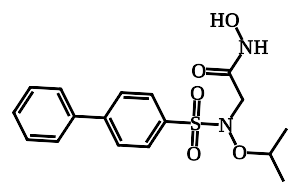
\includegraphics[width=3.2cm,height=0.9cm,keepaspectratio]{image/estruturas_ligantes_integracao/miniaturas/com_ARP_100.png} & Estrutura química consultada no PubChem \parencite{pubchem2023} \\
Ácido ascórbico & 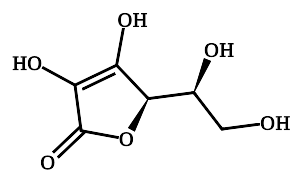
\includegraphics[width=3.2cm,height=0.9cm,keepaspectratio]{image/estruturas_ligantes_integracao/miniaturas/com_Acido_Ascorbico.png} & Estrutura química consultada no PubChem \parencite{pubchem2023} \\
Ácido kójico & 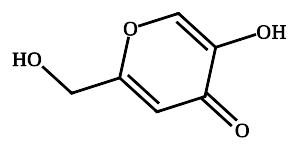
\includegraphics[width=3.2cm,height=0.9cm,keepaspectratio]{image/estruturas_ligantes_integracao/miniaturas/com_Acido_Kojico.png} & Estrutura química consultada no PubChem \parencite{pubchem2023} \\
Apigenina & 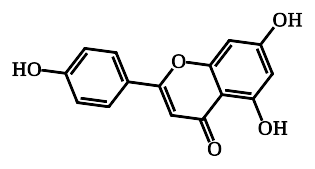
\includegraphics[width=3.2cm,height=0.9cm,keepaspectratio]{image/estruturas_ligantes_integracao/miniaturas/com_Apigenina.png} & Estrutura química consultada no PubChem \parencite{pubchem2023} \\
Arbutina & 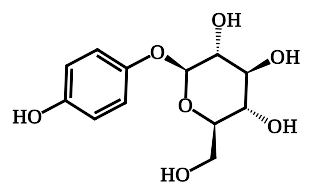
\includegraphics[width=3.2cm,height=0.9cm,keepaspectratio]{image/estruturas_ligantes_integracao/miniaturas/com_Arbutina.png} & Estrutura química consultada no PubChem \parencite{pubchem2023} \\
Batimastat & 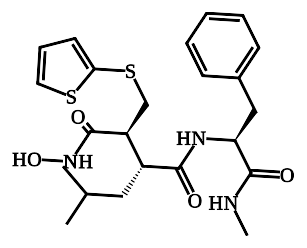
\includegraphics[width=3.2cm,height=0.9cm,keepaspectratio]{image/estruturas_ligantes_integracao/miniaturas/com_Batimastat.png} & Estrutura química consultada no PubChem \parencite{pubchem2023} \\
Cromoglicato & 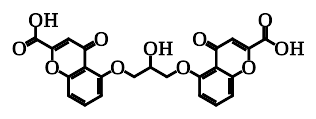
\includegraphics[width=3.2cm,height=0.9cm,keepaspectratio]{image/estruturas_ligantes_integracao/miniaturas/com_Cromoglicato.png} & Estrutura química consultada no PubChem \parencite{pubchem2023} \\
Doxiciclina & 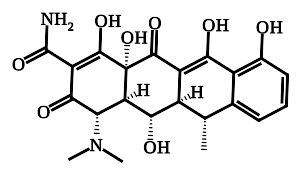
\includegraphics[width=3.2cm,height=0.9cm,keepaspectratio]{image/estruturas_ligantes_integracao/miniaturas/com_Doxiciclina.png} & Estrutura química consultada no PubChem \parencite{pubchem2023} \\
GW475151 & 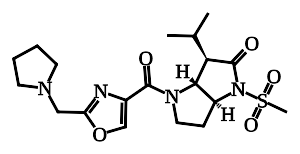
\includegraphics[width=3.2cm,height=0.9cm,keepaspectratio]{image/estruturas_ligantes_integracao/miniaturas/com_GW475151.png} & Complexo cristalográfico de elastase \parencite{macdonald2002} \\
Hidroquinona & 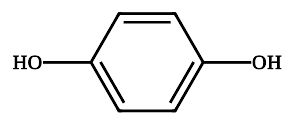
\includegraphics[width=3.2cm,height=0.9cm,keepaspectratio]{image/estruturas_ligantes_integracao/miniaturas/com_Hidroquinona.png} & Estrutura química consultada no PubChem \parencite{pubchem2023} \\
L2U & 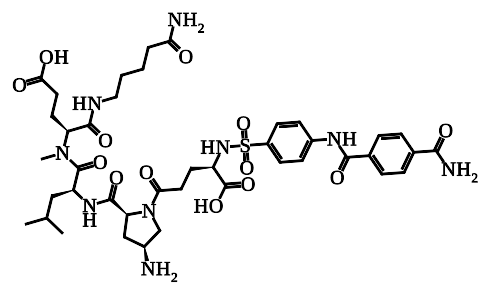
\includegraphics[width=3.2cm,height=0.9cm,keepaspectratio]{image/estruturas_ligantes_integracao/miniaturas/com_L2U.png} & Complexo cristalográfico de MMP-2 \parencite{takeuchi2023} \\
Marimastat & 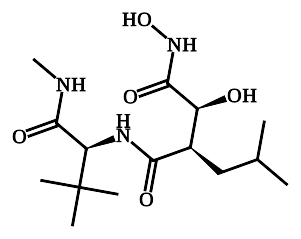
\includegraphics[width=3.2cm,height=0.9cm,keepaspectratio]{image/estruturas_ligantes_integracao/miniaturas/com_Marimastat.png} & Estrutura química consultada no PubChem \parencite{pubchem2023} \\
NFH & 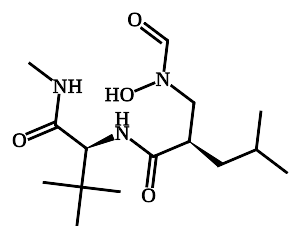
\includegraphics[width=3.2cm,height=0.9cm,keepaspectratio]{image/estruturas_ligantes_integracao/miniaturas/com_NFH.png} & Complexo cristalográfico de MMP-9 \parencite{rowsell2002} \\
PLH & 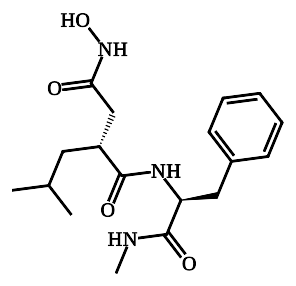
\includegraphics[width=3.2cm,height=0.9cm,keepaspectratio]{image/estruturas_ligantes_integracao/miniaturas/com_PLH.png} & Complexo cristalográfico de MMP-1 \parencite{spurlino1994} \\
Quercetina & 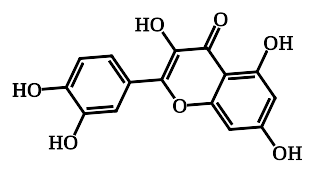
\includegraphics[width=3.2cm,height=0.9cm,keepaspectratio]{image/estruturas_ligantes_integracao/miniaturas/com_Quercetina.png} & Estrutura química consultada no PubChem \parencite{pubchem2023} \\
Sivelestat & 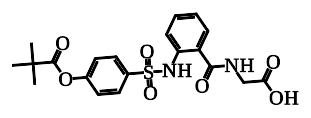
\includegraphics[width=3.2cm,height=0.9cm,keepaspectratio]{image/estruturas_ligantes_integracao/miniaturas/com_Sivelestat.png} & Estrutura química consultada no PubChem \parencite{pubchem2023} \\
Tropolona & 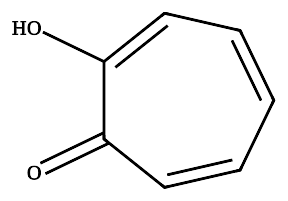
\includegraphics[width=3.2cm,height=0.9cm,keepaspectratio]{image/estruturas_ligantes_integracao/miniaturas/com_Tropolona.png} & Estrutura química consultada no PubChem \parencite{pubchem2023} \\
\end{longtable}
\normalsize
\renewcommand{\arraystretch}{1.25}
\setlength{\tabcolsep}{6pt}


\setlength{\LTpre}{\baselineskip}
\setlength{\LTpost}{6pt}
\small
\renewcommand{\arraystretch}{1.1}
\setlength{\tabcolsep}{3pt}
\begin{longtable}{C{3.4cm}C{3.7cm}C{7.0cm}}
\caption{Compostos selecionados para prospecção.}\label{tab:ligantes_spe_metodos}\\
\toprule Ligante & Estrutura bidimensional & Fonte da estrutura ou referência \\
\midrule
\endfirsthead
\multicolumn{3}{c}{\tablename~\thetable\ (continuação)}\\
\toprule Ligante & Estrutura bidimensional & Fonte da estrutura ou referência \\
\midrule
\endhead
\midrule
\multicolumn{3}{r}{Continua na próxima página}\\
\endfoot
\bottomrule
\endlastfoot
Ácido ferúlico & 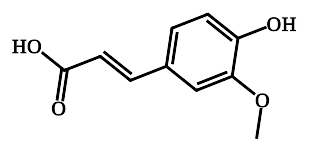
\includegraphics[width=3.2cm,height=0.9cm,keepaspectratio]{image/estruturas_ligantes_integracao/miniaturas/spe_Acido_Ferulico.png} & Extrato de biomassa de \textit{T. tetrahele} \parencite{mai2026} \\
Ácido galacturônico & 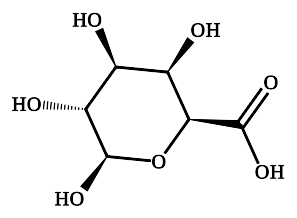
\includegraphics[width=3.2cm,height=0.9cm,keepaspectratio]{image/estruturas_ligantes_integracao/miniaturas/spe_Acido_Galacturonico.png} & Exopolissacarídeos de \textit{T. suecica} \parencite{parra2020} \\
Ácido gálico & 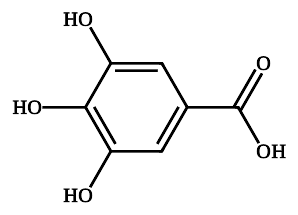
\includegraphics[width=3.2cm,height=0.9cm,keepaspectratio]{image/estruturas_ligantes_integracao/miniaturas/spe_Acido_Galico.png} & Extrato de biomassa de \textit{T. tetrahele} \parencite{mai2026} \\
Ácido glucurônico & 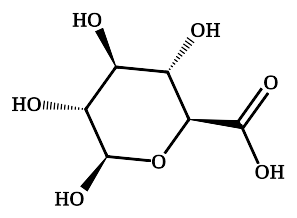
\includegraphics[width=3.2cm,height=0.9cm,keepaspectratio]{image/estruturas_ligantes_integracao/miniaturas/spe_Acido_Glucuronico.png} & Exopolissacarídeos de \textit{T. suecica} \parencite{parra2020} \\
D-Galactose & 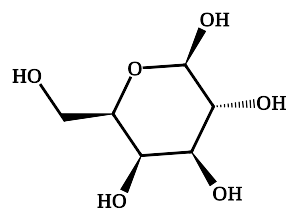
\includegraphics[width=3.2cm,height=0.9cm,keepaspectratio]{image/estruturas_ligantes_integracao/miniaturas/spe_D_Galactose.png} & Biomassa de \textit{T. chuii}; exopolissacarídeos de \textit{T. suecica} \parencite{brown1991,pereira2019,parra2020} \\
D-Glicose & 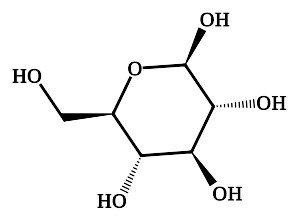
\includegraphics[width=3.2cm,height=0.9cm,keepaspectratio]{image/estruturas_ligantes_integracao/miniaturas/spe_D_Glicose.png} & Biomassa de \textit{T. chuii}; exopolissacarídeos de \textit{T. suecica} \parencite{brown1991,pereira2019,parra2020} \\
D-Gulose & 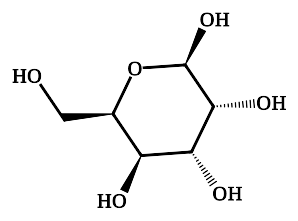
\includegraphics[width=3.2cm,height=0.9cm,keepaspectratio]{image/estruturas_ligantes_integracao/miniaturas/spe_D_Gulose_Raro_presente_na_SPE.png} & Parede celular de \textit{T. striata} \parencite{becker1989} \\
D-Manose & 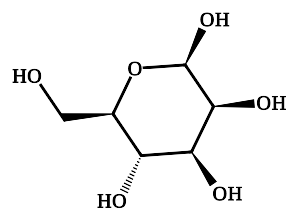
\includegraphics[width=3.2cm,height=0.9cm,keepaspectratio]{image/estruturas_ligantes_integracao/miniaturas/spe_D_Manose.png} & Biomassa de \textit{T. chuii}; exopolissacarídeos de \textit{T. suecica} \parencite{brown1991,pereira2019,parra2020} \\
D-Xilose & 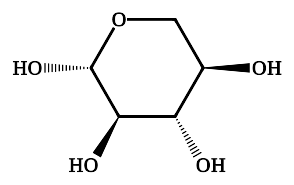
\includegraphics[width=3.2cm,height=0.9cm,keepaspectratio]{image/estruturas_ligantes_integracao/miniaturas/spe_D_Xilose.png} & Exopolissacarídeos de \textit{T. suecica} \parencite{parra2020} \\
\textit{Dha} & 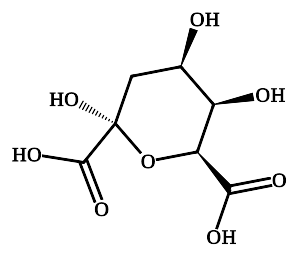
\includegraphics[width=3.2cm,height=0.9cm,keepaspectratio]{image/estruturas_ligantes_integracao/miniaturas/spe_Dha_3_deoxy_D_lyxo_hept_2_ulopyranosaric_acid.png} & Parede celular de \textit{T. striata} \parencite{becker1989} \\
Galactose-6-sulfato & 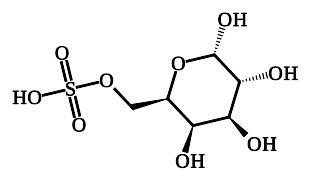
\includegraphics[width=3.2cm,height=0.9cm,keepaspectratio]{image/estruturas_ligantes_integracao/miniaturas/spe_Galactose_6_sulfato.png} & Comparador estrutural em galactanos de algas vermelhas (\textit{Gloiopeltis} e \textit{Acanthophora}); ocorrência em \textit{Tetraselmis} não identificada \parencite{tuvikene2015funorans,duarte2004} \\
Glicose-6-sulfato & 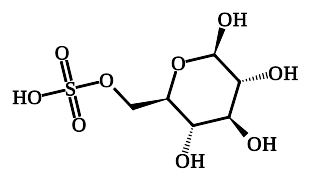
\includegraphics[width=3.2cm,height=0.9cm,keepaspectratio]{image/estruturas_ligantes_integracao/miniaturas/spe_Glicose_6_sulfato.png} & Em polissacarídeo sulfatado de \textit{T. suecica}, a sulfatação foi proposta no O-6 de resíduos de glicose \parencite{li2026tetraselmis} \\
KDO & 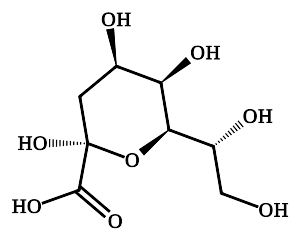
\includegraphics[width=3.2cm,height=0.9cm,keepaspectratio]{image/estruturas_ligantes_integracao/miniaturas/spe_KDO_3_deoxy_D_manno_oct_2_ulosonic_acid.png} & Parede celular de \textit{T. striata} \parencite{becker1989} \\
L-Arabinose & 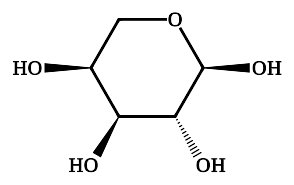
\includegraphics[width=3.2cm,height=0.9cm,keepaspectratio]{image/estruturas_ligantes_integracao/miniaturas/spe_L_Arabinose.png} & Biomassa de \textit{T. chuii}; exopolissacarídeos de \textit{T. suecica} \parencite{brown1991,pereira2019,parra2020} \\
L-Fucose & 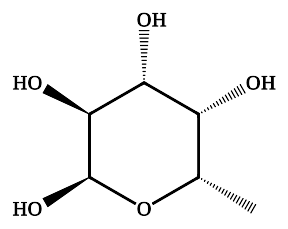
\includegraphics[width=3.2cm,height=0.9cm,keepaspectratio]{image/estruturas_ligantes_integracao/miniaturas/spe_L_Fucose.png} & Exopolissacarídeos de \textit{T. suecica} \parencite{parra2020} \\
L-Ramnose & 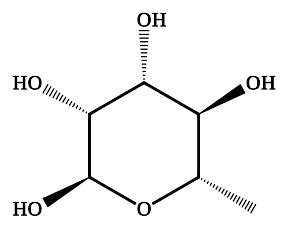
\includegraphics[width=3.2cm,height=0.9cm,keepaspectratio]{image/estruturas_ligantes_integracao/miniaturas/spe_L_Ramnose.png} & Biomassa de \textit{T. chuii}; exopolissacarídeos de \textit{T. suecica} \parencite{brown1991,pereira2019,parra2020} \\
$\alpha$-Kdo & 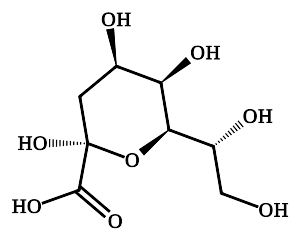
\includegraphics[width=3.2cm,height=0.9cm,keepaspectratio]{image/estruturas_ligantes_integracao/miniaturas/spe_alpha_Kdo_Isomero_comum_em_polissacarideos.png} & Comparador estrutural; sem fonte de ocorrência identificada \\
\end{longtable}
\normalsize
\renewcommand{\arraystretch}{1.25}
\setlength{\tabcolsep}{6pt}


A Tabela~\ref{tab:inventario} apresenta os 34 ligantes utilizados nas simulações, distribuídos entre os comerciais e coocristalizados e os compostos selecionados para prospecção de \textit{T. chuii}. Os códigos dos ligantes coocristalizados foram preservados para permitir a correspondência com os arquivos de entrada.

\begin{table}[H]
\centering\caption[Inventário dos 34 ligantes]{Inventário dos 34 ligantes: comerciais e coocristalizados e compostos selecionados para prospecção de \textit{T. chuii}.}\label{tab:inventario}
\begin{tabular}{C{7.0cm}C{7.0cm}}
\toprule \shortstack{Comerciais e coocristalizados\\($n=17$)} & \shortstack{Compostos para prospecção de \\\textit{T. chuii} ($n=17$)} \\\midrule
ARP-100 & Ácido ferúlico \\
Ácido ascórbico & Ácido galacturônico \\
Ácido kójico & Ácido gálico \\
Apigenina & Ácido glucurônico \\
Arbutina & D-Galactose \\
Batimastat & D-Glicose \\
Cromoglicato & D-gulose \\
Doxiciclina & D-Manose \\
GW475151 & D-Xilose \\
Hidroquinona & Dha \\
L2U & Galactose-6-sulfato \\
Marimastat & Glicose-6-sulfato \\
NFH & KDO \\
PLH & L-Arabinose \\
Quercetina & L-Fucose \\
Sivelestat & L-Ramnose \\
Tropolona & $\alpha$-Kdo \\
\bottomrule\end{tabular}
\fonte{Adaptado das referências citadas anteriormente no texto.}
\end{table}

A identificação de Dha, KDO e $\alpha$-Kdo foi conferida no inventário de preparação dos ligantes, que reúne nomes, SMILES e CIDs associados aos registros do PubChem. Dha corresponde ao CID 15608515, KDO ao CID 10857507 e $\alpha$-Kdo ao CID 445569. A conferência combinou esses identificadores com as informações de conectividade e estereoquímica e com as estruturas preparadas em PDBQT \parencite{pubchem2023}.

\subsection{Estruturas dos receptores e preparação dos arquivos}
Os receptores foram selecionados no Protein Data Bank (PDB), repositório de estruturas tridimensionais de proteínas e outras macromoléculas. A seleção considerou se a estrutura correspondia ao alvo humano desejado, o método de determinação, a resolução, a presença de ligante cristalográfico ou cofatores e a disponibilidade das coordenadas necessárias ao estudo \parencite{berman2000pdb}. Em seguida, o registro de cada estrutura foi conferido no RCSB (\textit{Research Collaboratory for Structural Bioinformatics}) PDB e comparado com o artigo associado. Essa conferência confirmou a identidade do alvo e os dados estruturais usados na preparação. A Tabela~\ref{tab:receptores} reúne o código PDB, o nome do receptor, a resolução reportada e a publicação correspondente.

\begin{table}[H]
\centering\caption[Estruturas dos receptores humanos]{Estruturas cristalográficas humanas utilizadas: código PDB, identidade do alvo, resolução e estudo de referência.}\label{tab:receptores}
\begin{tabular}{C{1.1cm}C{4.4cm}C{1.9cm}C{5.7cm}}
\toprule PDB & Alvo humano & Resolução (\AA) & Referência \\\midrule
1GKC & MMP-9 / gelatinase B & 2,30 & \textcite{rowsell2002} \\
1H1B & Elastase de neutrófilos & 2,00 & \textcite{macdonald2002} \\
1HFC & MMP-1 / colagenase & 1,50 & \textcite{spurlino1994} \\
2PE4 & Hialuronidase 1 & 2,00 & \textcite{chao2007} \\
5M8P & TYRP1 humana & 2,80 & \textcite{lai2017} \\
8H78 & MMP-2 / gelatinase A & 2,40 & \textcite{takeuchi2023} \\
\bottomrule\end{tabular}
\fonte{RCSB PDB, consulta em 5 out. 2026.}
\end{table}

A estrutura 5M8P corresponde à TYRP1 humana, determinada em complexo com tirosina, e contém dois íons de zinco em seu centro metálico \parencite{lai2017}. A TYRP1 foi incluída como alvo relacionado à pigmentação. As seis estruturas utilizadas apresentam resoluções entre 1,50 e 2,80~\AA.

\subsubsection{Preparação das estruturas tridimensionais dos ligantes}
Quando presentes, os ligantes coocristalizados foram extraídos dos mesmos arquivos PDB usados para obter os receptores. A separação preservou as coordenadas experimentais observadas no complexo e produziu um arquivo de ligante independente do arquivo proteico. Assim, cada ligante pôde ser preparado e submetido ao cálculo separadamente, enquanto sua pose cristalográfica permaneceu disponível para comparação. Os ligantes comerciais sem estrutura coocristalizada e os 17 compostos selecionados para prospecção de \textit{T. chuii} foram baixados do PubChem como estruturas tridimensionais no formato SDF (\textit{Structure Data File}). Os nomes, CIDs e representações SMILES foram conferidos em conjunto: o CID identifica o registro no PubChem, e o SMILES permite comparar as ligações entre átomos e a estereoquímica de cada estrutura \parencite{pubchem2023}.

Antes do \textit{docking}, cada ligante foi preparado em um arquivo PDBQT separado. Foram adicionados todos os átomos de hidrogênio para representar a protonação e os grupos capazes de doar ligações de hidrogênio, além de cargas parciais que aproximam a distribuição elétrica da molécula. No cálculo com AD4, essas cargas entram no termo eletrostático; a pontuação Vina não utiliza diretamente os valores de carga do arquivo e estima as interações por seus próprios termos. Também foram definidas as ligações rotacionáveis: o programa mantém a conectividade da molécula e pode variar a rotação em torno dessas ligações ao explorar poses. A posição e a orientação do ligante também são ajustadas durante a busca \parencite{morris2009autodock,trott2010,eberhardt2021vina}.

\subsubsection{Preparação dos receptores e mapas de afinidade}
Cada receptor foi preparado a partir do arquivo PDB correspondente. Quando havia ligante coocristalizado, ele foi separado da proteína para deixar o sítio de ligação disponível durante o cálculo. As águas cristalográficas foram removidas; os íons de zinco que integram os sítios ativos foram mantidos. Foram adicionados todos os átomos de hidrogênio e atribuídas cargas parciais, e a estrutura foi convertida para PDBQT, que registra coordenadas, tipos atômicos e cargas. Durante o \textit{docking}, cada receptor foi tratado como rígido, com as coordenadas proteicas fixas. A busca variou a posição e a orientação do ligante e suas ligações rotacionáveis, mantendo o receptor preparado como referência para todas as moléculas testadas naquele alvo \parencite{morris2009autodock,eberhardt2021vina}.

A função AD4 requer mapas de afinidade calculados antes da busca. Para MMP-1 (1HFC), MMP-2 (8H78), MMP-9 (1GKC) e TYRP1 (5M8P), os mapas foram preparados com a parametrização AD4Zn. Eles cobrem a região de busca por uma grade tridimensional; em cada ponto, o mapa armazena a contribuição energética de um tipo de átomo do ligante em relação ao receptor. Ao avaliar uma pose, o programa consulta os mapas correspondentes aos átomos do ligante. A parametrização AD4Zn ajusta os mapas para descrever a geometria e a energia da coordenação com zinco, componente relevante nos sítios ativos dessas quatro estruturas \parencite{morris2009autodock,santos2014zn}.

A elastase (1H1B) e a hialuronidase 1 (2PE4) foram avaliadas com a função de pontuação Vina. Nesse protocolo, o AutoDock Vina calcula internamente as grades usadas na busca; por isso, não foram necessários mapas AD4 ou AD4Zn preparados externamente. Em ambos os protocolos, as poses foram geradas pelo AutoDock Vina; a função de pontuação e a preparação das grades variaram conforme o receptor \parencite{eberhardt2021vina}.

A Figura~\ref{fig:fluxo_ferramentas} resume a sequência das ferramentas e a escolha da função de pontuação conforme a presença de zinco no sítio ativo.

\begin{figure}[H]
\centering
\captionsetup{justification=centering,singlelinecheck=false}
\caption[Fluxo das ferramentas de triagem]{Sequência das ferramentas e etapas da triagem computacional, da obtenção das estruturas à organização dos resultados.}
\label{fig:fluxo_ferramentas}
\begin{tikzpicture}[
    caixa/.style={draw=black!70,fill=black!8,rounded corners=4pt,
      text width=10.5cm,minimum height=1.05cm,inner sep=5pt,align=center,font=\footnotesize},
    ramificacao/.style={draw=black!70,fill=black!8,rounded corners=4pt,
      text width=5.1cm,minimum height=1.25cm,inner sep=5pt,align=center,font=\footnotesize},
    decisao/.style={diamond,aspect=2.5,draw=black!70,fill=black!8,
      text width=3.7cm,inner sep=2pt,align=center,font=\footnotesize},
    seta/.style={-{Stealth},thick,black!70}
  ]
    \node[caixa,text width=12.5cm] (fontes) at (0,0)
      {Obter as estruturas: receptores e ligantes coocristalizados no PDB; demais ligantes no PubChem};
    \node[caixa,text width=12.5cm] (preparo) at (0,-1.65)
      {Preparar os arquivos PDBQT: remover águas, adicionar todos os átomos de hidrogênio e cargas parciais, definir ligações rotacionáveis dos ligantes e manter os receptores rígidos};
    \node[decisao] (zn) at (0,-4.0) {O sítio ativo contém zinco?};
    \node[ramificacao] (ad4zn) at (-4.0,-5.75)
      {Com zinco: gerar mapas de afinidade AD4Zn e usar a pontuação AD4 com parâmetros para zinco};
    \node[ramificacao] (vina) at (4.0,-5.75)
      {Sem zinco: usar a função de pontuação Vina};
    \coordinate (uniao_busca) at (0,-7.05);
    \node[caixa] (busca) at (0,-7.9)
      {AutoDock Vina 1.2.7: buscar poses e calcular as pontuações com a função selecionada};
    \node[caixa] (feb) at (0,-9.55)
      {Selecionar a pose de menor FEB para cada combinação de receptor e ligante};
    \node[caixa] (plip) at (0,-11.2)
      {PLIP 2.3.0: analisar os relatórios e identificar os contatos entre ligante e receptor};
    \node[caixa] (pymol) at (0,-12.7)
      {PyMOL 2.5.0: inspecionar as poses selecionadas e gerar imagens dos complexos};
    \node[caixa] (tratamento) at (0,-14.2)
      {Tratar e organizar os resultados: FEB, RMSD, matriz de contatos, tabelas e gráficos};
    \node[caixa] (resultados) at (0,-15.7)
      {Comparar os resultados por receptor e apresentar a análise};

    \draw[seta] (fontes) -- (preparo);
    \draw[seta] (preparo.south) -- (zn.north);
    \draw[seta] (zn.west) -- (ad4zn.north);
    \draw[seta] (zn.east) -- (vina.north);
    \draw[thick,black!70] (ad4zn.south) |- (uniao_busca);
    \draw[thick,black!70] (vina.south) |- (uniao_busca);
    \fill[black!70] (uniao_busca) circle (1.2pt);
    \draw[seta] (uniao_busca) -- (busca.north);
    \draw[seta] (busca) -- (feb);
    \draw[seta] (feb) -- (plip);
    \draw[seta] (plip) -- (pymol);
    \draw[seta] (pymol) -- (tratamento);
    \draw[seta] (tratamento) -- (resultados);
  \end{tikzpicture}
\end{figure}

\subsection{Execução do docking e definição das regiões de busca}
Todas as simulações foram executadas no AutoDock Vina versão 1.2.7 \parencite{eberhardt2021vina}. O algoritmo explora posições, orientações e ligações rotacionáveis do ligante por busca estocástica, seguida de otimização local das poses. A função de pontuação Vina combina contribuições de ajuste estérico, interações hidrofóbicas e ligações de hidrogênio, além de considerar a flexibilidade do ligante \parencite{trott2010,eberhardt2021vina}. O AutoDock Vina também permite selecionar a função AD4. Assim, o algoritmo propõe e otimiza as poses, enquanto a função escolhida calcula a pontuação de cada pose.

Para 1GKC, 1HFC, 5M8P e 8H78, a opção de comando \texttt{--scoring ad4} selecionou a pontuação AD4, utilizando mapas de afinidade AD4Zn. Para 1H1B e 2PE4, empregou-se a função Vina com os receptores em formato PDBQT. A função AD4 combina contribuições de van der Waals, ligações de hidrogênio, eletrostática, dessolvatação e uma penalização associada aos graus de liberdade torsionais do ligante \parencite{morris2009autodock}. Assim, a principal diferença entre os protocolos está na função que calcula a FEB e no tratamento do receptor, embora ambos usem o AutoDock Vina para buscar as poses.

O AD4Zn estende a função AD4 para representar a coordenação de ligantes com zinco. Utiliza potenciais de Lennard--Jones 12--6 parametrizados para os tipos atômicos envolvidos, com distância de equilíbrio e intensidade calibradas para cada par metal--coordenante. A parametrização trata especificamente oxigênio aceptor e enxofre e representa a direcionalidade do nitrogênio aceptor por pseudoátomos tetraédricos do tipo TZ. A carga parcial do zinco é definida como zero na componente eletrostática; os potenciais calibrados descrevem sua coordenação com os ligantes \parencite{santos2014zn}. Na TYRP1 (5M8P), a configuração dos mapas considerou o centro binuclear de zinco descrito na estrutura cristalográfica \parencite{lai2017}.

Na execução anterior, mantida para os outros quatro receptores, foi utilizado \textnormal{exhaustiveness 64}. Os demais parâmetros registrados foram \textnormal{num\_modes 9}, \textnormal{energy\_range 3}, \textnormal{cpu 2}, \textnormal{spacing 1}~\AA{} e \textnormal{seed 0}. O parâmetro \textnormal{exhaustiveness} estabelece o esforço de exploração do espaço conformacional; \textnormal{num\_modes} limita a nove o número máximo de poses armazenadas; \textnormal{energy\_range} restringe a saída a poses situadas em uma faixa de até 3~kcal/mol em relação à melhor pontuação; \textnormal{cpu} define o uso de dois núcleos de processamento; \textnormal{spacing} fixa em 1~\AA{} a separação entre os pontos da grade; e \textnormal{seed 0} solicita a geração de uma semente para a execução. A solicitação de nove modos corresponde a um limite máximo e não exige que todas as combinações produzam nove poses \parencite{autodockvina_manual}. Nas execuções atualizadas de 1H1B e 2PE4, os registros de comando indicam \texttt{energy\_range=100}~kcal/mol e \texttt{min\_rmsd=0.5}~\AA, com \texttt{exhaustiveness=64}, \texttt{num\_modes=9}, \texttt{cpu=2}, \texttt{seed=0} e espaçamento de 1~\AA{}.

As análises de contatos utilizaram relatórios em XML (\textit{Extensible Markup Language}) do PLIP versão 2.3.0 \parencite{salentin2015plip} associados às poses dos complexos. Para 1H1B e 2PE4, foram usados os resultados atualizados com coordenadas corrigidas para os dois grupos. A pose de menor FEB foi conferida nos arquivos PDBQT e na tabela da execução; o relatório correspondente forneceu os dados para a matriz de contatos.


A Tabela~\ref{tab:caixas} reúne os centros e tamanhos definidos para as caixas de busca dos ligantes comerciais e de referência e dos compostos selecionados para prospecção. Nos casos com pontuação AD4, esses limites espaciais foram associados aos mapas de afinidade pré-calculados utilizados pelo programa.

\begin{table}[H]
\centering\caption[Caixas de busca por receptor]{Centro e dimensões das caixas de busca utilizadas no docking dos dois grupos; todas as coordenadas e dimensões estão em angströms (\AA).}\label{tab:caixas}
\begin{tabular}{C{1.8cm}C{6.2cm}C{4.9cm}}
\toprule Receptor & Centro $(x,y,z)$, em \AA & Tamanho $(x,y,z)$, em \AA \\\midrule
1H1B & 17,756; 13,110; 21,780 & 20,000; 20,000; 22,000 \\
1GKC & 65,401; 31,636; 118,169 & 32,000; 22,000; 30,000 \\
8H78 & 28,361; 23,813; -6,701 & 32,000; 28,000; 34,000 \\
2PE4 & 44,979; -31,339; -3,339 & 40,000; 40,000; 40,000 \\
1HFC & 23,281; 23,363; 25,811 & 22,000; 26,000; 22,000 \\
5M8P & 31,529; 136,753; 216,460 & 40,000; 40,000; 44,000 \\
\bottomrule\end{tabular}
\fonte{Parâmetros do protocolo de docking.}
\end{table}

O espaçamento entre os pontos da grade foi fixado em 1~\AA{} para todos os receptores. A Tabela~\ref{tab:mapas} apresenta somente a função de pontuação correspondente a cada estrutura: Vina para 1H1B e 2PE4 e AD4 com mapas AD4Zn para os quatro receptores com tratamento específico para zinco.

\begin{table}[H]
\centering\caption[Funções de pontuação por receptor]{Função de pontuação adotada por receptor.}\label{tab:mapas}
\begin{tabular}{C{3.5cm}C{8.0cm}}
\toprule Receptor & Função de pontuação \\\midrule
1H1B & Vina \\
2PE4 & Vina \\
1GKC & AD4 com mapas AD4Zn \\
1HFC & AD4 com mapas AD4Zn \\
5M8P & AD4 com mapas AD4Zn \\
8H78 & AD4 com mapas AD4Zn \\
\bottomrule\end{tabular}
\fonte{Parâmetros do protocolo de docking.}
\end{table}

As imagens da Figura~\ref{fig:receptores_caixas} mostram a posição dos ligantes coocristalizados em relação às caixas definidas na Tabela~\ref{tab:caixas}. Para a estrutura 2PE4, que não contém ligante coocristalizado, apresenta-se o receptor com a caixa de busca.

\begin{figure}[H]
\centering
\captionsetup{justification=centering,singlelinecheck=false}
\caption[Receptores, ligantes coocristalizados e caixas de busca]{Receptores com os ligantes coocristalizados e as caixas posicionadas conforme os centros e dimensões da Tabela~\ref{tab:caixas}.}
\label{fig:receptores_caixas}
\begin{minipage}{0.48\linewidth}\centering
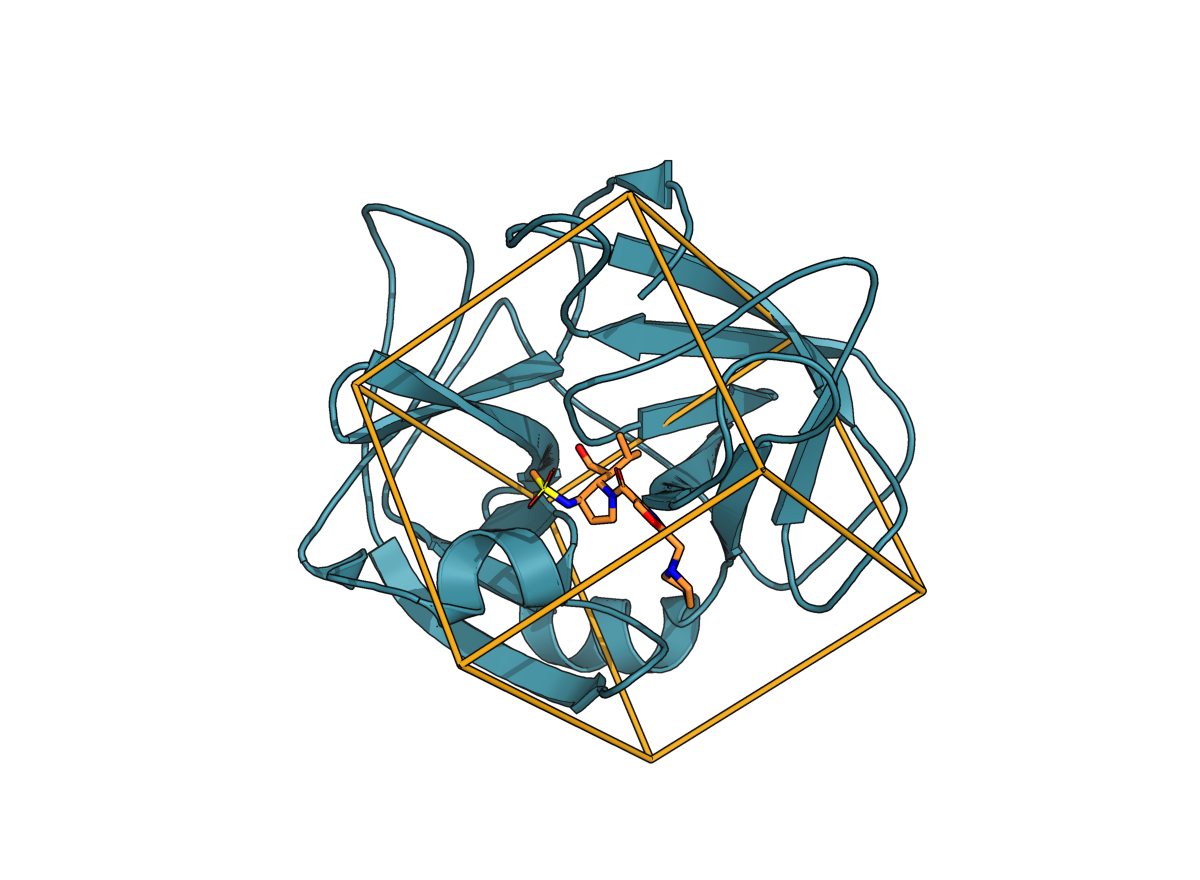
\includegraphics[width=\linewidth]{image/caixas_receptores/png/1H1B_caixa.png}\\[-1mm]
\small (a) Elastase (1H1B) — ligante 151
\end{minipage}\hfill
\begin{minipage}{0.48\linewidth}\centering
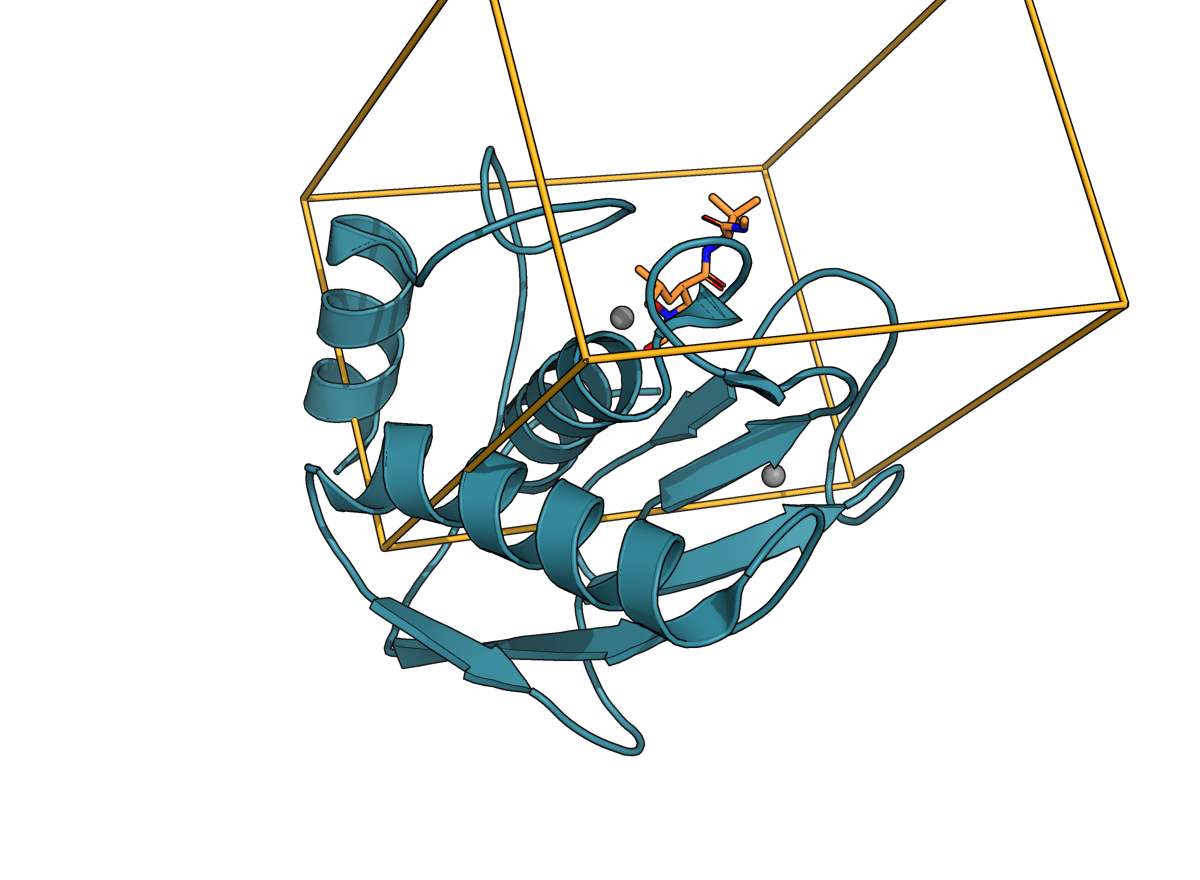
\includegraphics[width=\linewidth]{image/caixas_receptores/png/1GKC_caixa.png}\\[-1mm]
\small (b) MMP-9 (1GKC) — ligante NFH
\end{minipage}\par\vspace{1mm}
\begin{minipage}{0.48\linewidth}\centering
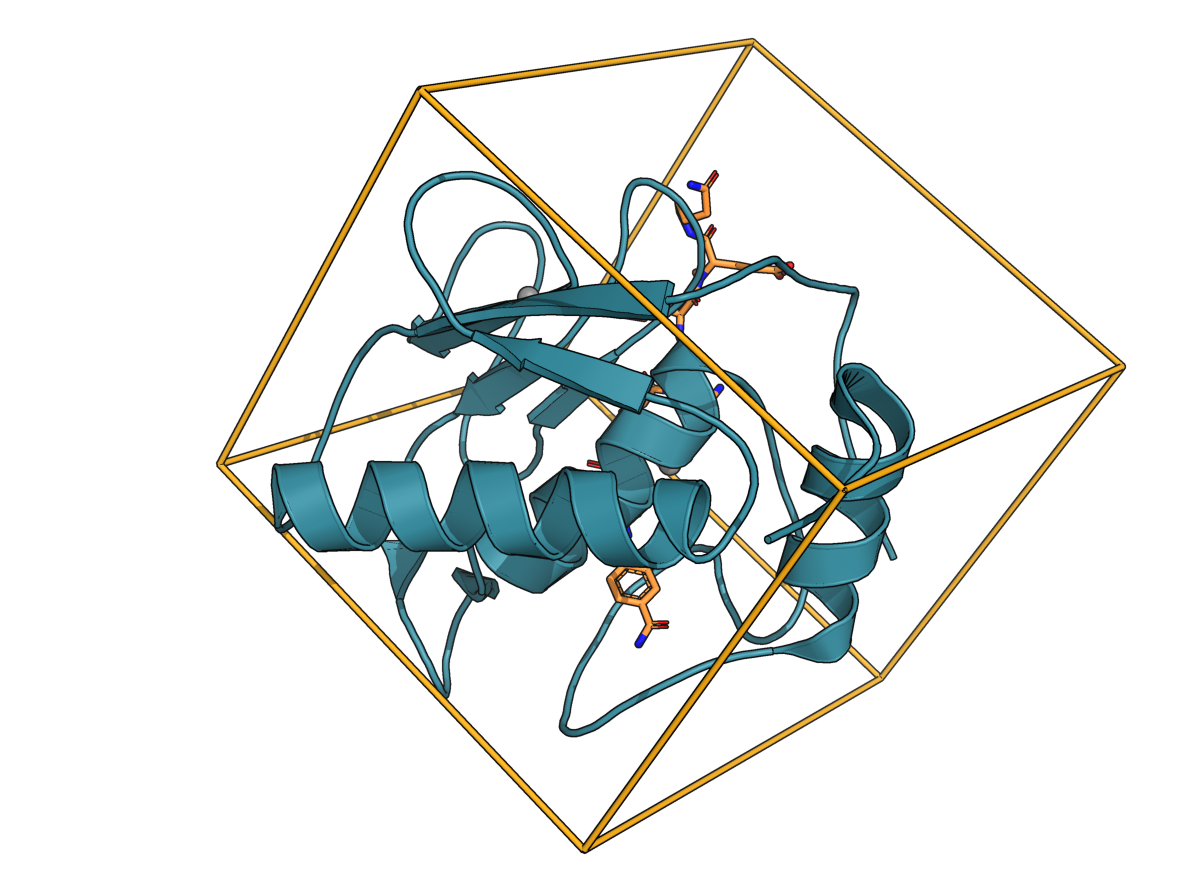
\includegraphics[width=\linewidth]{image/caixas_receptores/png/8H78_caixa.png}\\[-1mm]
\small (c) MMP-2 (8H78) — ligante L2U
\end{minipage}\hfill
\begin{minipage}{0.48\linewidth}\centering
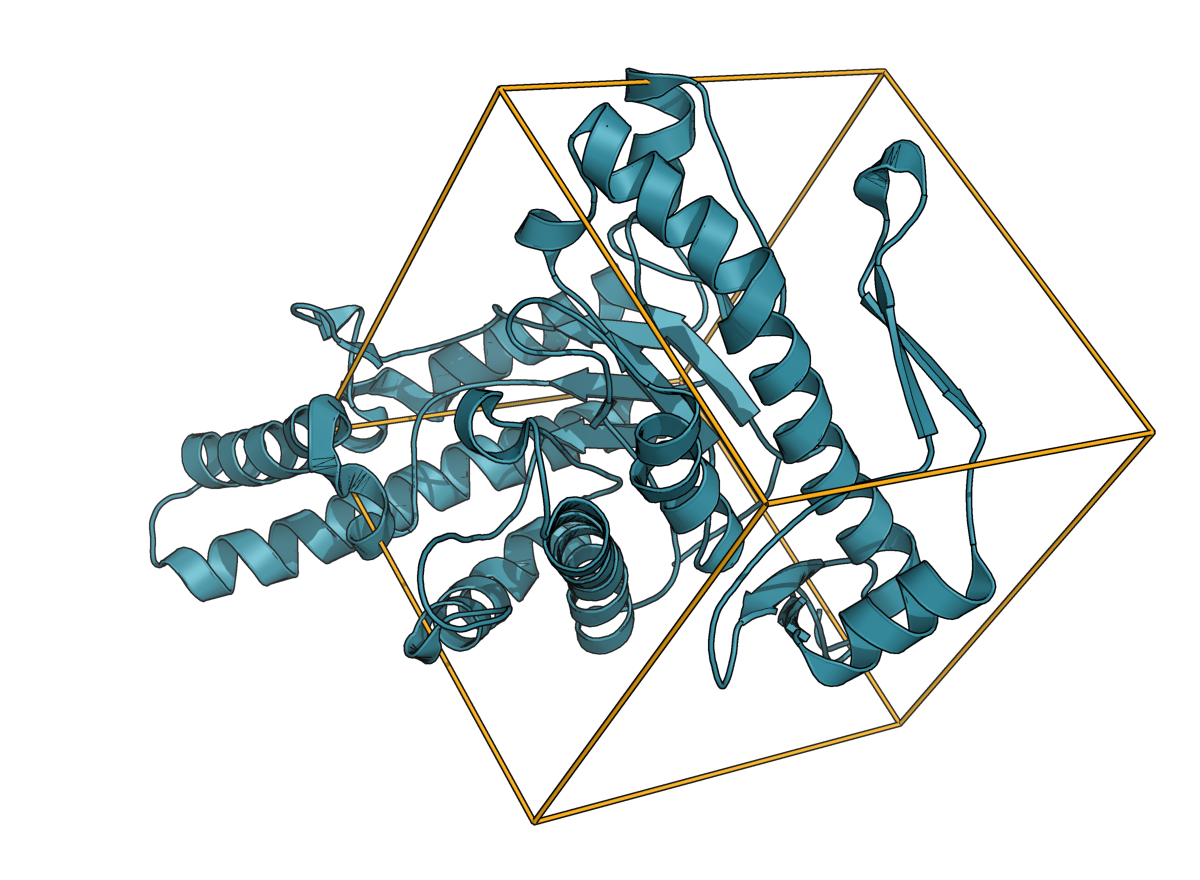
\includegraphics[width=\linewidth]{image/caixas_receptores/png/2PE4_caixa.png}\\[-1mm]
\small (d) Hialuronidase 1 (2PE4) — sem ligante coocristalizado
\end{minipage}\par\vspace{1mm}
\begin{minipage}{0.48\linewidth}\centering
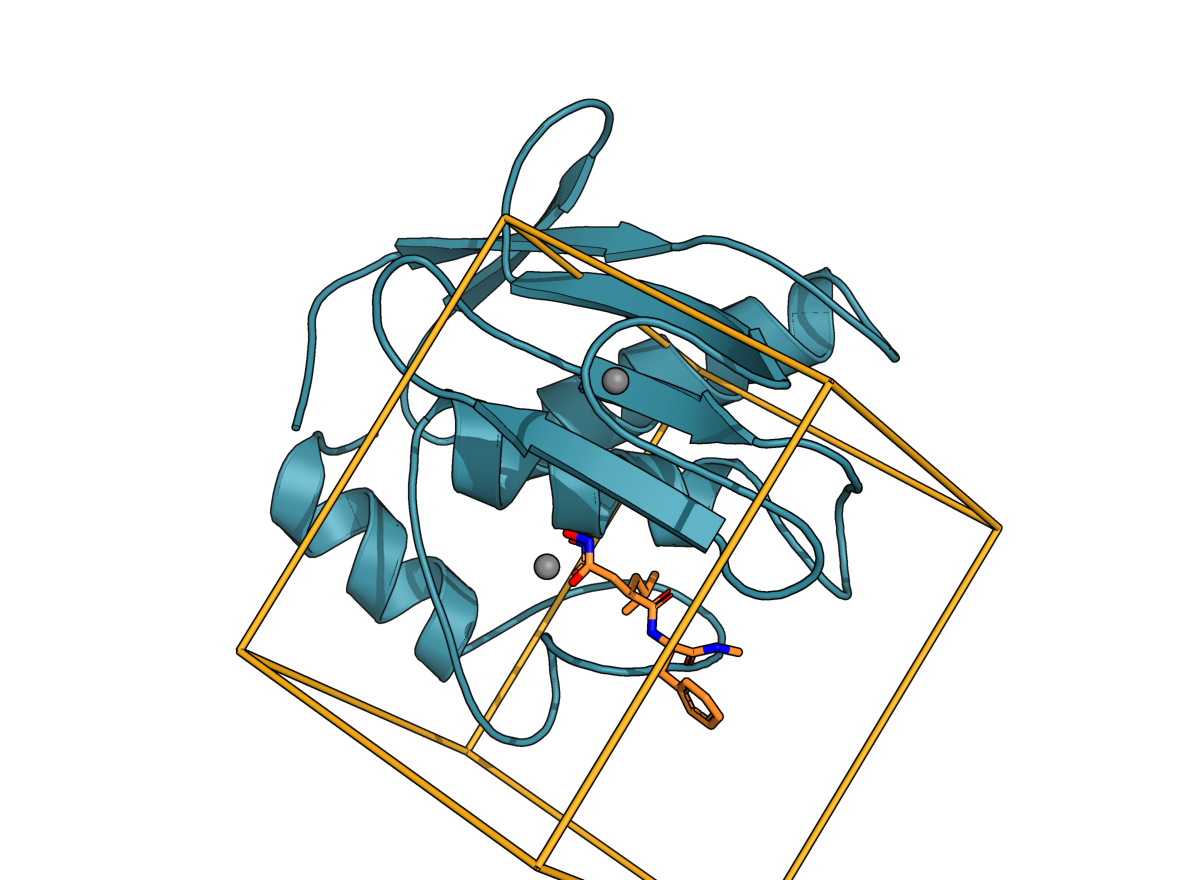
\includegraphics[width=\linewidth]{image/caixas_receptores/png/1HFC_caixa.png}\\[-1mm]
\small (e) MMP-1 (1HFC) — ligante PLH
\end{minipage}\hfill
\begin{minipage}{0.48\linewidth}\centering
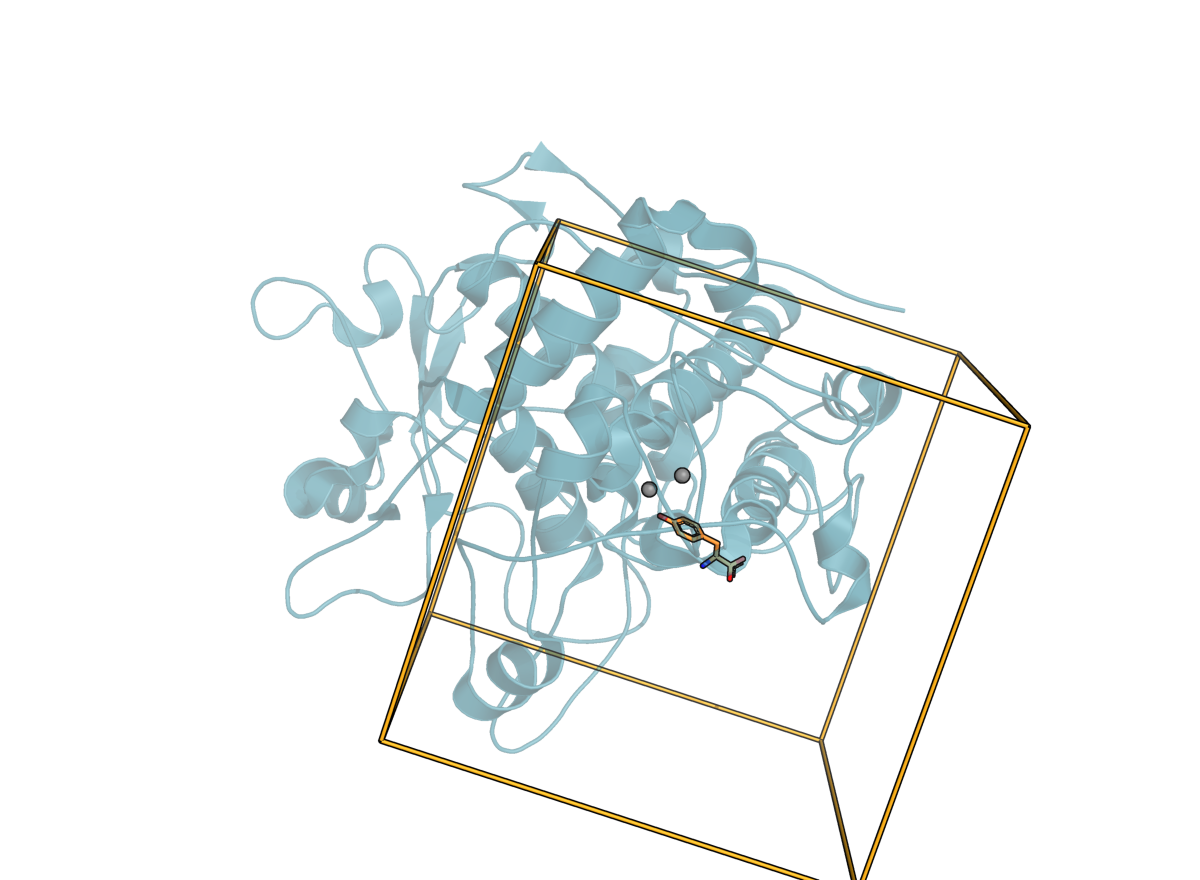
\includegraphics[width=\linewidth]{image/caixas_receptores/png/5M8P_caixa.png}\\[-1mm]
\small (f) TYRP1 (5M8P) — tirosina
\end{minipage}
\fonte{Estruturas do RCSB Protein Data Bank; imagens geradas no PyMOL 3.2.0a0 com ray tracing \parencite{pymol}. Proteínas em cartoon azul-esverdeado, ligantes em bastões laranja e caixas em amarelo.}
\end{figure}

\subsection{Seleção por FEB e análise das interações}
Para cada combinação receptor--ligante, selecionou-se a pose com a menor FEB, expressa em kcal/mol. A FEB é a pontuação calculada pela função adotada; valores mais negativos indicam poses mais bem avaliadas pelo modelo. A comparação dos ligantes foi feita dentro de cada receptor, considerando a função e as condições de execução correspondentes \parencite{trott2010,eberhardt2021vina,warren2006}.

As interações previstas entre os ligantes e os resíduos dos receptores foram extraídas com o PLIP versão 2.3.0, a partir dos relatórios em XML (\textit{Extensible Markup Language}) e dos arquivos de texto simples (TXT) gerados pela ferramenta \parencite{salentin2015plip}. Nos arquivos, o código UNL identifica os ligantes sem nome padronizado; os resíduos são identificados por nome, número e cadeia. Para montar os mapas, cada par ligante--resíduo foi contado uma vez. Os gráficos apresentam o número de ligantes distintos por resíduo e de resíduos distintos por ligante. As coordenações metal--receptor em sítios separados foram mantidas fora dessas contagens, e a origem dos relatórios foi registrada.

Para a comparação final em cada receptor, selecionou-se o ligante de menor FEB do conjunto de 17 ligantes comerciais e coocristalizados. Entre os 17 compostos para prospecção, escolheu-se aquele que compartilhou o maior número de resíduos de contato com esse ligante. Em caso de empate, prevaleceu o composto com FEB mais negativa. Assim, a seleção considerou primeiro a sobreposição dos contatos e, em seguida, a pontuação calculada.

\subsection{Comparação com ligantes cristalográficos e cálculo de RMSD}
Foram avaliadas as referências NFH/1GKC, GW475151/1H1B, PLH/1HFC, L-tirosina/5M8P e L2U/8H78. A L-tirosina foi utilizada somente nessa análise estrutural suplementar e não integrou os 34 ligantes da triagem. Para 2PE4 não havia ligante cristalográfico equivalente disponível para essa comparação. O RMSD foi utilizado como medida geométrica da semelhança conformacional após ajuste independente do ligante \parencite{cole2005}.

Para $N$ pares de átomos correspondentes, o desvio foi expresso por:
\begin{equation}
\label{eq:rmsd}
\mathrm{RMSD}=\sqrt{\frac{1}{N}\sum_{i=1}^{N}\|\mathbf{x}_{i}-\mathbf{y}_{i}\|^2}.
\end{equation}
Na Equação~\ref{eq:rmsd}, $N$ representa o número de pares de átomos correspondentes e $\mathbf{x}_i$ e $\mathbf{y}_i$ são suas coordenadas no ligante na pose obtida pelo \textit{docking} e na referência cristalográfica, respectivamente. O RMSD é expresso em angströms. O ajuste independente aplica rotação e translação aos ligantes para minimizar o desvio e avaliar a semelhança entre suas conformações \parencite{cole2005}.

Selecionou-se o menor RMSD entre átomos pesados correspondentes após ajuste independente, mantendo esse critério separado da seleção por FEB.



\subsection{Preparação das figuras e organização dos resultados}
As imagens de sobreposição dos ligantes foram geradas no PyMOL 2.5.0 por \textit{ray tracing}, em 1800~$\times$~1200 pixels \parencite{pymol}. As imagens dos receptores e das caixas de busca (Figura~\ref{fig:receptores_caixas}) foram renderizadas com PyMOL 3.2.0a0, também por \textit{ray tracing}, em 1200~$\times$~880 pixels. Nas sobreposições dos ligantes isolados, a referência cristalográfica aparece em verde e a pose prevista pelo \textit{docking} em laranja. As correspondências entre átomos pesados foram obtidas com RDKit 2024.03.5 \parencite{rdkit}, incluindo equivalências de grupos terminais conjugados quando aplicáveis, e conferidas pela reprodução dos RMSDs da análise consolidada. O ajuste rígido foi aplicado com \textnormal{pair\_fit} do PyMOL aos pares de átomos correspondentes. Essa transformação gerou as imagens conformacionais; as análises de FEB e de contatos utilizaram as poses originais.

Os painéis bidimensionais dos ligantes são apresentados no \hyperref[ap:estruturas_ligantes]{Apêndice~B}. Para essas representações, utilizaram-se o RDKit 2025.09.4 e os SMILES registrados nos arquivos PDBQT das execuções atualizadas, sem modificar os arquivos das simulações.

\subsection{Apoio à organização textual}
O ChatGPT, da OpenAI, acessado pelo plano ChatGPT Plus, foi utilizado como apoio à organização da estrutura textual e à revisão da clareza da redação (OpenAI, 2026). A seleção das fontes e a versão final do conteúdo são de responsabilidade do autor.
